
\chapter{Computing Roots Over Finite Fields}
\label{chapter:rootcomp}

Let $R$ be a ring and let $a \in R$. Computing $a^{1/n}$, where $n$ is an integer, beside its 
intrinsic interest, is of great importance in many areas of mathematics and computer science. This 
problem can equivalently be considered as finding a root of $x^n - a \in R[x]$ in some extension of 
$R$. In this chapter, we focus on the cases where $R$ is a finite field, and devote some more space 
to the case $n = 2$ which is of special interest in point counting and cryptography. The first two 
sections are preliminary for subsequent sections. We first present some square root algorithms, and 
then extend them to compute higher roots.



\section{Discrete logarithm in cyclic $p$-groups}
\label{section:dlp-cpgroups}

A finite $p$-group $G$ is a group of order $n = p^m$ where $p$ is a prime. A special case of the 
discrete logarithm problem occurring in root computation is the one in finite cyclic $p$-groups. The 
algorithm we present here is due to Pohlig and Hellman \cite{Pohlig1978}. Let $g, a \in G$ with $g$ 
a generator of $G$. The problem is to find the integer $0 \le x \le n - 1$ such that $g^x = a$. 
Suppose that $x$ has the expansion $x = \sum_{i = 0}^{m - 1}x_ip^i, \: 0 \le x_i \le p - 1$ in base 
$p$. Then
\begin{equation}
\label{equation:dlp-dh}
a^{\frac{n}{p}} = g^{x\frac{n}{p}} = (g^{\frac{n}{p}})^x = (g^{\frac{n}{p}})^{\sum_{i = 0}^{m - 
1}x_ip^i} = (g^{\frac{n}{p}})^{x_0} = \zeta^{x_0}
\end{equation}
where $\zeta = g^{\frac{n}{p}}$ is a primitive $p$-th root of unity. Therefore, $x_0$ is uniquely 
determined by (\ref{equation:dlp-dh}). Let assume $x_1, \dots, x_k, \: k < m$ are determined. Then 
$$
(ag^{-\sum_{i = 0}^{k}x_ip^i})^{n / p^{k + 2}} = (g^{\frac{n}{p}})^{x_{k + 2}} = \zeta^{x_{k + 2}}
$$
so that $x_{k + 1}$ is uniquely determined, and hence $x$ is determined by induction. When $p$ is 
small, the values $0 \le x_i \le p - 1$ can be found by a brute force search. But when $p$ is large, 
one can use techniques like Shank's baby-step giant-step \cite{Shank1971} and Pollard's rho method 
\cite{Pollard1978}. The baby-step giant-step algorithm needs memory for $O(\sqrt{p})$ group 
elements, and its running time is $O(\sqrt{p})$ group multiplications; while the running time of the 
Pollard's rho method is the same, but it requires a negligible amount of memory. The expected 
running time of the above algorithm, which requires $m$ exponentiations and applications of, say 
Pollard's method, for discrete logarithm in $G$ is $O(m(\log_2{n} + \sqrt{p}))$ group 
multiplications.







\section{Randomized search for irreducible polynomials}
\label{section:r-s-irr-poly}

In this section, we briefly discuss the asymptotic probability for a randomly selected polynomial, 
with prescribed constraints, to be irreducible over a finite field. Let $N(n, q)$ denote the number 
of monic irreducible polynomials of degree $n$ over $\vmathbb{F}_q$. It is not hard to prove that 
$$
N(n, q) = \frac{1}{n}\sum_{d \mid n}\mu(d)q^{\frac{n}{d}}
$$
where $\mu$ is the M\"obius function. This formula was discovered by Gauss \cite{Gauss1981} for the 
case $q = p$. There are $q^n$ monic polynomials of degree $n$ over $\vmathbb{F}_q$. So, the 
probability $P(n, q)$ for a uniformly random monic polynomial of degree $n$ to be irreducible is 
$N(n, q) / q^n$. The following lemma shows that $P(n, q) \in \Theta(\frac{1}{n})$.
\begin{lemma}
The number $N(n, q)$ of monic irreducible polynomials of degree $n$ over $\vmathbb{F}_q$ satisfies
$$
\frac{1}{n}q^n - \frac{q}{n(q - 1)}(q^{\frac{n}{2}}) \le N(q, n) \le \frac{1}{n}(q^n - q) \qquad n 
\ge 2
$$
with equality on the right if and only if $n$ is prime.
\end{lemma}
\begin{proof}
The equality on the right is trivial when $n$ is prime. By the M\"obius inversion 
$$
q^n = \sum_{d \mid n}dN(d, q) = nN(n, q) + q + \sum_{\substack{d \mid n \\ d \ne 1, n}}dN(d, q) \ge 
nN(n, q) + q
$$
which establishes the upper bound. Once we proved the upper bound it can be used to prove the lower 
bound:
\begin{align*}
q^n = \sum_{d \mid n}dN(d, q) 
&= nN(n, q) + \sum_{\substack{d \mid n \\ d \ne n}}dN(d, q) \\
&\le nN(n, q) + \sum_{d = 1}^{n / 2} q^d = nN(n, q) + q \frac{q^{\frac{n}{2}} - 1}{q - 1} \qedhere
\end{align*}
\end{proof}
The coefficient of $x^{n - 1}$ of the monic polynomial $f$ of degree $n$ is called the trace of $f$. 
Let $N_\gamma(n, q)$ denote the number of polynomials of degree $n$ and trace $\gamma$ over 
$\vmathbb{F}_q$. Carlitz \cite{Carlitz1952} showed that
$$
N_\gamma(n, q) = \frac{1}{qn}\sum_{\substack{d \mid n \\ p \nmid d}} \mu(d)q^{\frac{n}{d}} \qquad 
\gamma \ne 0
$$
which means that $N_\gamma(n, q)$ does not depend on the trace $\gamma$. Let $n = p^km$ with $p 
\nmid m$. Then 
$$
N_0(n, q) = \frac{1}{qn}\sum_{d \mid m} \mu(d)q^{\frac{n}{d}} - \frac{\varepsilon}{n}\sum_{d \mid 
m}\mu(d)q^{\frac{n}{dp}} \qquad \gamma \ne 0
$$
where $\varepsilon = 1$ if $k > 0$ and $\varepsilon = 0$ if $k = 0$ \cite{Yucas2006}. Let $N(n, c, 
q)$ denote the number of monic irreducible polynomial of degree $n$ and constant term $c$. Let $D_n 
= \{r : r \mid q^n - 1, r \nmid q^m - 1 \text{ for } m < n\}$, and let $\lambda$ be the order of 
$c$. For each $r \in D_n$ let $r = m_rd_r$ where $d_r = \gcd(r, (q^n - 1)/(q - 1))$. An explicit 
formula for $N(n, c, q)$ was obtained in \cite{Yucas2006} as follows.
\begin{equation}
\label{equation:irr-const}
N(n, c, q) = \frac{1}{n\varphi(\lambda)}\sum_{\substack{r \in D_n \\ m_r = \lambda}} \varphi(r)
\end{equation}
where $\varphi$ is the Euler's function. Following the same notation as above let $N_\gamma(n, c, 
q)$ denote the number of irreducible polynomials of degree $n$, trace $\gamma$, and constant term 
$c$. The following bound was established by Wan \cite{Wan1997}. See \cite{Moisio2007} for an 
improvement to this bound.
\begin{equation}
\label{equation:irr-const-bound}
\left| N_\gamma(n, c, q) - \frac{q^{n - 1}}{n(q - 1)}\right| \le \frac{3}{n}q^{n / 2}
\end{equation}
Let $P(n, c, q)$ denote the probability for a uniformly random monic polynomial of degree $n$ and 
constant term $c$ to be irreducible. 
Summing both sides of (\ref{equation:irr-const}) over all elements of $\vmathbb{F}_q$ we have
\begin{align*}
\frac{3}{n}q^{(n + 2) / 2} = \sum_{\gamma \in \vmathbb{F}_q}\frac{3}{n}q^{n / 2} 
& \ge \sum_{\gamma \in \vmathbb{F}_q} \left| N_\gamma(n, c, q) - \frac{q^{n - 1}}{n(q - 1)}\right| \\
& \ge \left| \sum_{\gamma \in \vmathbb{F}_q}N_\gamma(n, c, q) - \sum_{\gamma \in 
\vmathbb{F}_q}\frac{q^{n - 1}}{n(q - 1)}\right| \\
& = \left| N(n, c, q) - \frac{q^n}{n(q - 1)}\right|
\end{align*}
Since the number of all polynomials of degree $n$ and a prescribed constant term is $q^{n - 1}$, the 
above bound shows that $P(n, c, q) \in \Theta(\frac{1}{n})$. This means that for a monic polynomial 
$f \in \vmathbb{F}_q[x]$ of degree $n$, if the constant term is fixed and all other coefficients are 
selected in a uniformly random way then there still is a reasonable chance for $f$ to be 
irreducible. The surprising fact is that the above asymptotic results hold for some polynomials of 
very special form. Extensive research has been done on the number of irreducible binomials and 
trinomials over finite fields. These polynomials are very computationally useful, and result in 
simpler representations of extensions of finite fields. 

Let $T_n(p)$ be the number of irreducible polynomials of the form $x^n + x + a \in \vmathbb{F}_p[x]$ 
over $\vmathbb{F}_p$. Then $T_n(p)$ is asymptotic to $p / n$ for a fixed $n$ and $p \rightarrow 
\infty$. This was first conjectured by Chowla \cite{Chowla1966}. The following more general result 
was proved by Cohen \cite{Cohen1970} and Ree \cite{Ree1971}. 
\begin{theorem}
For an integer $n$ such that $p \nmid n(n - 1)$, let $T_n(q)$ denote the number of trinomials $x^n + 
x + a \in \vmathbb{F}_q[x]$ that are irreducible over $\vmathbb{F}_q$. Then
$$
\left| T_n(q) - \frac{q}{n} \right| \le C_nq^{\frac{1}{2}}
$$
where $C_n$ is a constant depending only on $n$.
\end{theorem}









\section{General approaches}

There are many polynomial factorization algorithms that can be used as general algorithms to find an 
$n$th root of an element of a finite field. See \cite{vonzurGathen2001} for a survey of polynomial 
factorization over finite fields and \cite{Lidl-Niederreiter1994} for special root finding 
algorithms based on factorization. For an element $a \in \vmathbb{F}_q$ if $\sqrt[n]{a} \notin 
\vmathbb{F}_q$ then there is a finite extension $\vmathbb{F}_{q^m} / \vmathbb{F}_q$ containing 
$\sqrt[n]{a}$. Therefore, given $a \in \vmathbb{F}_q$, we can always assume that an $n$-th root of 
$a$ is contained in $\vmathbb{F}_q$, since a polynomial over $\vmathbb{F}_q$ can always be viewed as a 
polynomial over $\vmathbb{F}_{q^m}$. Let $f \in \vmathbb{F}_q[x]$ be an arbitrary polynomial. To find 
the zeros of $f$ in $\vmathbb{F}_q$, it is sufficient to apply the equal degree factorization 
algorithm to $\gcd(x^q - x, f)$.

\begin{algorithm}
[Root finding using factorization]
\label{algorithm:groot1}
\begin{algorithmic}[1]
\REQUIRE A nonconstant $f \in \vmathbb{F}_q[x]$
\ENSURE  Zeros of $f$ in $\vmathbb{F}_q$
\STATE $h \leftarrow x^q \mod f$.
\label{step:genroot-pow}
\STATE $g \leftarrow \gcd(h - x, f), d \leftarrow \deg{g}$
\label{step:genroot-gcd}
\IF {$d = 0$} 
	\RETURN $\varnothing$
\ENDIF
\STATE factorize $g$ using equal degree factorization to get the linear factors $x - u_i, \: i = 1, 
\dots, d$
\RETURN $u_i, \: i = 1, \dots, d$
\end{algorithmic}
\end{algorithm}

\refalgorithm{algorithm:groot1} can be applied to the polynomial $x^n - a$ to compute an $n$-th root 
of $a$. It is essentially due to Legendre \cite{Legendre1785}. He suggested, in the case $q = p$, 
splitting $\gcd(f, x^{p - 1} - 1)$ by computing $\gcd(f, x^{(p - 1) / 2} \pm 1)$ and substituting 
$x$ by $x + a$ for a random $a \in \vmathbb{F}_p$ in the case of a trivial split. The dominant steps 
of the algorithm are steps \ref{step:genroot-pow} and \ref{step:genroot-gcd} which take 
$O(M(n)\log{q})$ and $O((\log{q} + \log{n})M(n)\log{n})$ operations in $\vmathbb{F}_q$ respectively. 
Therefore, the running time is $O(M(n)\log{n}\log(nq))$ or $\tilde{O}(n\log{q})$ operations in 
$\vmathbb{F}_q$.








\section{Computing square roots}
\label{section:squareroot}

Let $G$ be a group with an odd order $n$. Then the mapping $f: G \rightarrow G$, $f(x) = x^2$ is an 
automorphism of $G$, hence every element $x \in G$ has a unique square root which is $x^{(n + 
1)/2}$. For the cyclic group $\vmathbb{F}_q^*$ if $q = 2^m$ then the square root of $x \in 
\vmathbb{F}_q^*$ is $x^{2^{n - 1}}$. In fact, this is true in general, i.e. for $q = p^n$ the $p$-th 
root of $x \in \vmathbb{F}_q^*$ is $x^{p^{n - 1}}$. If $q \equiv 3 \pmod 4$ then for any $x \in 
(\vmathbb{F}_q^*)^2$ the square root is $x^{(q + 1) / 4}$. The latter is because $(\vmathbb{F}_q^*)^2$ 
is a subgroup of odd order $(q - 1) / 2$.

An interesting field theoretic approach to computing square roots in $\vmathbb{F}_q$ was introduced 
by Cipolla \cite{Cipolla1903}. Let $K = \vmathbb{F}_{q^m}$ be a finite extension of $\vmathbb{F}_q$, 
and let $N_{K/\vmathbb{F}_q}: K \rightarrow \vmathbb{F}_q$ be the norm function 
$N_{K/\vmathbb{F}_q}(\alpha) = \prod_{i = 1}^{m - 1}\alpha^{q^i} = \alpha^{(q^m - 1)/(q - 1)}$. Then 
$N_{K/\vmathbb{F}_q}$ is surjective. The idea of Cipolla's algorithm is as follows. Let $a \in 
\vmathbb{F}_q$, and assume we find a quadratic extension $K = \vmathbb{F}_{q^2}$ of $\vmathbb{F}_q$ by 
adjoining a quadratic nonresidue to $\vmathbb{F}_q$. Then, there is an element $x \in K$ such that 
$N_{K/\vmathbb{F}_q}(x) = a$. But $N_{K/\vmathbb{F}_q}(x) = x^{q + 1}$ hence $\sqrt{a} = x^{(q + 1) / 
2}$.

\begin{algorithm}
[Cipolla's square root]
\label{algorithm:Cipolla-sq}
\begin{algorithmic}[1]
\REQUIRE A nonzero $a \in \vmathbb{F}_q$
\ENSURE Square root of $a$ in $\vmathbb{F}_{q^2}$
\STATE choose a random $b \in \vmathbb{F}_q$
\IF {$b^2 - 4a$ is a square} 
	\RETURN failure.
\ENDIF
\STATE $c \leftarrow x^{(q + 1) / 2} \mod x^2 - bx + a$
\label{step:Cipolla-norm}
\RETURN $c$
\end{algorithmic}
\end{algorithm}

If $\left( \frac{b^2 - 4a}{\vmathbb{F}_q}\right) = -1$ then the polynomial $f(x) = x^2 - bx + a$ is 
irreducible over $\vmathbb{F}_q$ hence $\vmathbb{F}_q[x]/(f)$ is a field. Since $f$ is the minimal 
polynomial of $x$ over $\vmathbb{F}_q$, $c^2 = N_{K/\vmathbb{F}_q}(x) = a$. According to 
\refsection{section:r-s-irr-poly}, finding a quadratic nonresidue of the form $b^2 - 4a$ by choosing 
random $b \in \vmathbb{F}_q$, which is equivalent to choosing a uniformly random polynomial of degree 
$2$ and constant term $a$, does not require too many trials. More precisely \cite[page 
158]{BachSh1996},

\begin{lemma}
The probability of $\left(\frac{b^2 - 4a}{\vmathbb{F}_q}\right) = -1$ for a randomly chosen $b \in 
\vmathbb{F}_q$ is $(q - 1)/2q$.
\end{lemma} 

\refalgorithm{algorithm:Cipolla-sq} fails with probability $(q + 1) / 2q$. The quadratic residue 
test, and \refstep{step:Cipolla-norm} take $O(\log q)$ and $O(\log q)$ multiplications in 
$\vmathbb{F}_q$ respectively. Therefore, its expected complexity is $O(\log q)$ multiplications in 
$\vmathbb{F}_q$.

Another algorithm for computing square roots is the algorithm of Tonelli \cite{Tonelli1891}. The 
algorithm, which is more group theoretic, was improved by Shanks \cite{Shanks1972} and is known as 
Tonelli-Shanks algorithm. The idea of the algorithm is to use discrete logarithm to reduce the 
problem to a subgroup of $\vmathbb{F}_q^*$ of an odd order. Let $q - 1 = 2^r\ell$ with $(\ell, 2) = 
1$. Let $H$ be the unique subgroup of $\vmathbb{F}_q^*$ of order $\ell$. Then we have a chain of 
subgroups
$$
H = H_0 \subset H_1 \subset \cdots \subset H_r = \vmathbb{F}_q^*
$$
where $H_i / H_{i - 1}$ is a simple group of order 2 for $i = 1, \dots, r$. The natural homomorphism 
$\vmathbb{F}_q^* \rightarrow \vmathbb{F}_q^* / H$ sends any quadratic nonresidue of $\vmathbb{F}_q^*$ 
to a generator of $\vmathbb{F}_q^* / H$. Assume we find a quadratic nonresidue $g \in 
\vmathbb{F}_q^*$. Then the square root of an element $a \in \vmathbb{F}_q^*$ can be computed as 
follows. We can be express $a$ as $g^th \in g^tH$ by solving a discrete logarithm in $\vmathbb{F}_q^* 
/ H$. Now, $t$ is necessarily even, so that $\sqrt{a} = g^{t / 2}h^{(\ell + 1) / 2}$. Here is the 
algorithm.

\begin{algorithm}
[Tonelli-Shanks square root]
\label{algorithm:Tonelli-sq}
\begin{algorithmic}[1]
\REQUIRE A nonzero $a \in \vmathbb{F}_q$ with $q$ odd
\ENSURE Square root of $a$ in $\vmathbb{F}_{q}$
\STATE choose a random $g \in \vmathbb{F}_q$
\IF {$g$ is a square} 
	\RETURN failure.
\ENDIF
\STATE let $q - 1 = 2^r\ell$ with $2 \nmid \ell$.
\label{step:factor-q}
\STATE let $H$ be the subgroup of $\vmathbb{F}_q^*$ of order $\ell$
\STATE $t \leftarrow $ the discrete logarithm of $aH$ in base $gH$
\label{step:TS-DL}
%\FOR {$i = 2$ \TO $r$}
%	\IF {$(ag^{-t})^{(q - 1) / 2^i} \ne 1$} 
%		\STATE $t \leftarrow 2^{i - 1} + t$ 
%	\ENDIF
%\ENDFOR
\STATE $h \leftarrow ag^{-t}$
\RETURN $g^{t / 2}h^{(\ell + 1) / 2}$
\end{algorithmic}
\end{algorithm}

According to \refsection{section:dlp-cpgroups}, \refstep{step:TS-DL} of 
\refalgorithm{algorithm:Tonelli-sq} requires $O(r^2)$ multiplications in $\vmathbb{F}_q$ where $r$ is 
the highest power of $2$ dividing $q - 1$. All other steps take $O(\log q)$ multiplications in 
$\vmathbb{F}_q$. Hence, the expected running time of the algorithm is $O(r^2 + \log q)$ 
multiplications in $\vmathbb{F}_q$. Despite  \refalgorithm{algorithm:Cipolla-sq}, the efficiency of 
this algorithm depends on the structure of $\vmathbb{F}_q^*$. Let $r$ and $\ell$ be as in 
\refstep{step:factor-q} of the algorithm. For most $q$, $r$ is fairly small \footnote{For example, 
primes used in public-key cryptography, see \cite{Maurer1992a, Maurer1989}.}, and 
\refalgorithm{algorithm:Tonelli-sq} requires few exponentiations in $\vmathbb{F}_q^*$, and hence 
preferred over \refalgorithm{algorithm:Cipolla-sq} which requires exponentiation in 
$\vmathbb{F}_{q^2}$. If $2^r$ is comparable to $\ell$ then the running time of 
\refalgorithm{algorithm:Tonelli-sq} is $O((\log q)^2)$. In this case,  
\refalgorithm{algorithm:Cipolla-sq} is preferable. The latter case can happen quite naturally:
\begin{theorem}
\label{theorem:Dir-ar-prog}
Let $a$ and $b$ be positive coprime integers. Then there are infinitely many primes $p$ such that $p 
\overset{b}{\equiv} a$.
\end{theorem}

This is due to Dirichlet \cite{Dirichlet1837}, and known as \emph{Dirichlet's theorem on arithmetic 
progressions}; Because it equivalently says that if $a$ and $b$ are positive coprime integers then 
the arithmetic progression $a, a + b, a + 2b, \dots$ contains infinitely many primes. Let $p(a, b)$ 
be the least prime in this arithmetic progression. Linnik \cite{Linnik1944} proved that there is a 
constant $L > 0$ such that $p(a, b) < b^L$. This constant is not too large, e.g. it is shown in 
\cite{Heath-Brown1992} that $L \le 11/2$. By  \reftheorem{theorem:Dir-ar-prog}, for any given 
integer $r > 0$, there are infinitely many primes in the progression $1, 1 + 2.2^r, 1 + 3.2^r, 
\dots, 1 + k.2^r, \dots$. Let $q$ be the least prime in this sequence. Then $2^r \mid q - 1$, and $q 
\le 2^{11r/2}$, and hence $2\log q / 11 \le r$. This shows the bound $O((\log q)^2)$ for 
\refalgorithm{algorithm:Tonelli-sq} is tight.

Let $\mathcal{P} = \bigcup_{i \in \vmathbb{N}}\left\lbrace \text{the least prime } p_i \text{ such 
that } p_i \equiv 2^i + 1 \text{ mod } 2^{i + 1} \right\rbrace$. Then $\mathcal{P}$ is clearly not 
finite. Let $\{q_n\}_{n \in \vmathbb{N}}$ be an increasing sequence of elements of $\mathcal{P}$, and 
let $C(q)$ and $T(q)$ be the expected complexity of algorithms \ref{algorithm:Cipolla-sq} and 
\ref{algorithm:Tonelli-sq} respectively, averaged over all quadratic residue and non-residue inputs. 
Then it is not hard to prove, see \cite{Tornaria2002}, that
$$
\lim_{n \to \infty}\frac{T(q_n)}{C(q_n)} = \infty.
$$
which means we have found an infinite sequence of primes for which 
\refalgorithm{algorithm:Cipolla-sq} is asymptotically better.

The last square root algorithm we present is a new algorithm based on the trace function. Assume 
that the field $\vmathbb{F}_q$, where $q = p^n$, is represented, as usual, by a quotient 
$\vmathbb{F}_p[x] / (f(x))$ with $f(x) \in \vmathbb{F}_p[x]$ a monic irreducible polynomial of degree 
$n$. Let $T_{\vmathbb{F}_q / \vmathbb{F}_p}: \vmathbb{F}_q \rightarrow \vmathbb{F}_p$ be the trace 
function $T_{\vmathbb{F}_q / \vmathbb{F}_p}(\alpha) = \sum_{i = 0}^{n - 1} \alpha^{p^i}$ where $\alpha 
\in \vmathbb{F}_q$ . Given $a \in \vmathbb{F}_q^\times$, let $\gamma \in \vmathbb{F}_q$ be a square 
root of it. Then
\begin{equation}
\label{equation:tr-square}
\begin{aligned}
\vmathbb{F}_p \ni \beta = T_{\vmathbb{F}_q / \vmathbb{F}_p}(\gamma) = \sum_{i = 1}^{n - 1} \gamma^{p^i}
& = \gamma(1 + \gamma^{p - 1} + \gamma^{p^2 - 1} + \cdots + \gamma^{p^{n - 1} -1}) \\
& = \gamma(1 + a^{(p - 1) / 2} + a^{(p^2 - 1) / 2} + \cdots + a^{(p^{n - 1} -1) / 2})
\end{aligned}
\end{equation}
Let $b = 1 + a^{(p - 1) / 2} + a^{(p^2 - 1) / 2} + \cdots + a^{(p^{n - 1} -1) / 2}$. We may assume 
$b \ne 0$; because otherwise,  we can start by $ac^2$ for different random elements $c \in 
\vmathbb{F}_q^\times$ until we get a nonzero $b$, and at the end multiply the result by $c^{-1}$. 
Squaring both side of the \refequation{equation:tr-square} results in the quadratic equation 
$\beta^2 = ab^2$ over $\vmathbb{F}_p$ from which $\beta$ can be determined. Then $\gamma = \beta 
b^{-1}$. Computing $\beta$ from the above quadratic equation takes $O(\log p)$ operation in 
$\vmathbb{F}_p$. Therefore, efficient computation of $\gamma$ needs an efficient computation of $b$. 
For this, we use a recursive technique, similar to the one used in  \refsection{section:MMapll}, as 
follows. Let $\lambda \in \vmathbb{F}_q$, and assume we are asked to compute 
$$
\alpha_k = \lambda^{1 + p} + \lambda^{1 + p + p^2} + \cdots + \lambda^{1 + p + p^2 + \cdots + p^k}
$$
for a given integer $k > 0$. Let $\delta_i = \lambda^{p} + \lambda^{p + p^2} + \cdots + \lambda^{p + 
p^2 + \cdots + p^i}$, $\zeta_i = \lambda^{p + p^2 + \cdots + p^i}$, and $\xi_i = x^{p^i}$. Then we 
have the following recurrence relations
$$
\delta_i = 
\begin{cases}
\delta_{i / 2} + \zeta_{i / 2}\delta_{i / 2}^{p^{i / 2}} & \text{if } i \overset{2}{\equiv} 0 \\
\delta_1 + \zeta_1\delta_{i - 1}^p & \text{if } i \overset{2}{\equiv} 1 \\
\delta_1 = \lambda^p
\end{cases}
\qquad
\zeta_i = 
\begin{cases}
\zeta_{i / 2}\zeta_{i / 2}^{p^{i / 2}} & \text{if } i \overset{2}{\equiv} 0 \\
\zeta_1\zeta_{i - 1}^p & \text{if } i \overset{2}{\equiv} 1 \\
\zeta_1 = \lambda^p
\end{cases}
\qquad
\xi_i =
\begin{cases}
\xi_{i / 2}^{p^{i / 2}} & \text{if } i \overset{2}{\equiv} 0 \\
\xi_{i - 1}^p & \text{if } i \overset{2}{\equiv} 1 \\
\xi_1 = x^p
\end{cases}
$$
Assume, inductively, that we have computed $\delta_r$, $\zeta_r$, and $\xi_r$. Then $\delta_r^{p^r} 
= \left( \sum_{j = 0}^{n - 1} a_jx^j \right)^{p^r} = \sum_{j = 0}^{n - 1} a_j(x^j)^{p^r} = \sum_{j = 
0}^{n - 1} a_j(x^{p^r})^j = \sum_{j = 0}^{n - 1} a_j\xi_r^j$ which means that raising $\delta_r$ to 
the power of $p^r$ is indeed computing the modular polynomial composition $\delta_r\circ\xi_r$ over 
$\vmathbb{F}_p$. Thus, ignoring the additions, computing $\delta_{2r}$ and $\delta_{2r + 1}$ costs 
$O(1)$ polynomial multiplications and modular polynomial compositions over $\vmathbb{F}_p$. The same 
can be done for computing $\zeta_{2r}$, $\zeta_{2r + 1}$, $\xi_{2r}$, and $\xi_{2r + 1}$. Therefore, 
$\delta_k$ and hence $\alpha_k = \lambda\delta_k$ can by computed using $O(C(n)\log k)$ operations 
in $\vmathbb{F}_p$. Now, let $\lambda = a^{(p - 1) / 2}$, then $b = 1 + \lambda + \alpha_{n - 2}$. 
Computing $\lambda$ needs $O(M(n)\log p)$ operations in $\vmathbb{F}_p$, and hence computing $b$ 
needs $O(M(n)\log p + C(n)\log n)$ operations in $\vmathbb{F}_p$. Thus, the expected running time of 
the above algorithm for computing a square of an element $a \in \vmathbb{F}_q$ is $O(M(n)\log p + 
C(n)\log n)$ operations in $\vmathbb{F}_p$. 

\begin{figure}[ht]
\setlength{\abovecaptionskip}{-0.5cm}
%\setlength{\belowcaptionskip}{0cm}
\begin{center}
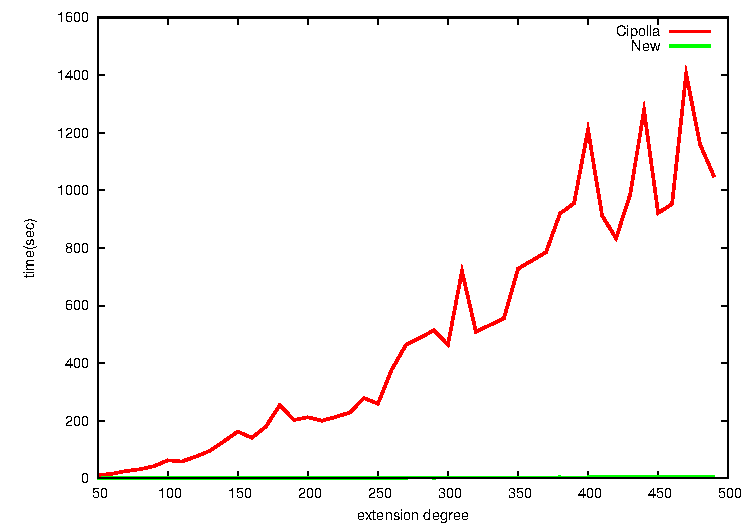
\includegraphics[width = 10cm]{figures/sqrtTiming.pdf}
\end{center}
\caption{\small The new square root algorithm}
\label{figure:sqrtTiming}
\end{figure}

We have implemented the above algorithm, and \refalgorithm{algorithm:Cipolla-sq} in NTL. Figure 
\ref{figure:sqrtTiming} compares the two algorithms in $\vmathbb{F}_q$ with $q = p^n$, for a randomly 
selected prime $p = \seqsplit{348975609381470925634534573457497}$, and different values of the 
extension degree $n$. Since Figure \ref{figure:sqrtTiming} does not reveal the behaviour of the new 
algorithm, a better view of the asymptotic  description of the algorithm for extension degrees $\le 
10000$ is provided in Figure \ref{figure:sqrtTimingHDeg}.

\begin{figure}[ht]
\setlength{\abovecaptionskip}{-0.5cm}
%\setlength{\belowcaptionskip}{0cm}
\begin{center}
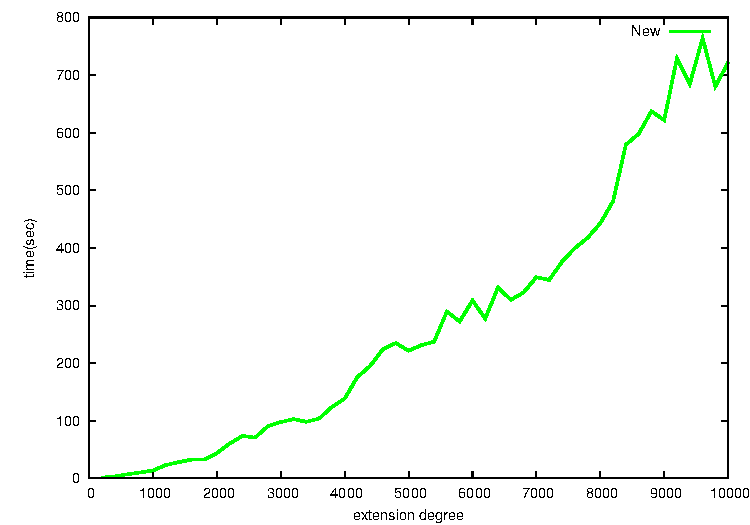
\includegraphics[width = 10cm]{figures/sqrtTimingHDeg.pdf}
\end{center}
\caption{\small The new square root algorithm for high extensions}
\label{figure:sqrtTimingHDeg}
\end{figure}










\section{Computing higher roots}

All of the algorithms presented in \refsection{section:squareroot} for computing square roots can 
somehow be extended to compute $m$-th roots where $m \ge 3$ is an arbitrary integer. In this 
section, we present such extensions, but let us first make the following observation. Let $G$ be a 
group of order $n$ and let $k$ be an integer such that $(n, k) = 1$. Then every $a \in G$ has a 
unique $k$-th root $b = a^{k^{-1} \text{ mod } n}$ in $G$; for if $c$ is another $k$-th root of $a$ 
then $b^k = c^k$ so $(cb^{-1})^k = 1$ which implies $\text{ord}(cb^{-1}) \mid k$ hence 
$\text{ord}(cb^{-1}) \mid (k, n) = 1$. Therefore $cb^{-1} = 1$ hence $c = b$. Suppose we can find a 
$t$-th root of $a \in \vmathbb{F}_q$ when $t$ is a prime divisor of $q - 1$. Then computing an $m$-th 
root of $a$ for an arbitrary $m$ is as follows. Let $m = m_1m_2$ with $(m_2, q - 1) = 1$, and $t 
\mid q - 1$ for every prime divisor $t$ of $m_1$. Then we can compute $a_0 = \sqrt[m_2]{a}$ by 
simply inverting $m_2 \text{ mod } q - 1$. Let $m_1 = \prod_{i = 1}^s{p_i^{\alpha_i}}$ be the prime 
factorization of $m_1$. Then we can compute $a_k = \sqrt[p_1]{a_{k - 1}},\: k = 1, \dots, \alpha_1$ 
and hence $a_{\alpha_1} = \sqrt[p_1^{\alpha_1}]{a_0}$. The same process can be applied to compute 
$\sqrt[p_2^{\alpha_2}]{a_{\alpha_1}}$ and so on. Therefore, the problem is reduced to computing 
$t$-th roots when $t$ is a prime divisor of $q - 1$, and so the algorithms we present in this 
section will compute $t$-th roots for such a $t$.

A natural extension of \refalgorithm{algorithm:Tonelli-sq} was introduced in \cite{AdlManMil1977}. 
Let $t$ be a prime divisor of $q - 1$ and let $q - 1 = t^r\ell$ such that $t \nmid \ell$. As before, 
let $H$ be the unique subgroup of $\vmathbb{F}_q^*$ of order $\ell$. Then we have a chain of 
subgroups
$$
H = H_0 \subset H_1 \subset \cdots \subset H_r = \vmathbb{F}_q^*
$$

where $H_i / H_{i - 1}$ is a simple group of order $t$ for $i = 1, \dots, r$. If $g$ is not a $t$-th 
power then $gH$ generates $\vmathbb{F}_q^*/H$ so that $a$ can be represented as $g^sh$ with $h \in 
H$. Since $a$ is a $t$-th power, it can easily be seen that $t \mid s$. On the other hand $(\left| H 
\right|, t) = 1$. Therefore, a $t$-th root of $a$ is $g^{s/t}h^{t^{-1} \text{ mod } \ell}$. 

\begin{algorithm}
[Tonelli-Shanks $t$-th root when $t$ is a prime divisor of $q - 1$]
\label{algorithm:AMM}
\begin{algorithmic}[1]
\REQUIRE A nonzero $a \in \vmathbb{F}_q$ with $q$ odd
\ENSURE a $t$-th root of $a$ in $\vmathbb{F}_{q}$
\STATE choose a random $g \in \vmathbb{F}_q$
\IF {$g$ is a $t$-th power} 
	\RETURN failure.
\ENDIF
\STATE let $q - 1 = t^r\ell$ with $t \nmid \ell$.
\STATE let $H$ be the subgroup of $\vmathbb{F}_q^*$ of order $\ell$
\STATE $s \leftarrow $ the discrete logarithm of $aH$ in base $gH$
\label{step:AMM-dlog}
\STATE $h \leftarrow ag^{-s}$
\STATE $u \leftarrow t^{-1} \text{ mod } \ell$
\RETURN $g^{s / t}h^u$
\end{algorithmic}
\end{algorithm}

By the following lemma, a randomly chosen $g \in \vmathbb{F}_q$ is a $t$-th power with probability 
$1/t$. Therefore, \refalgorithm{algorithm:AMM} fails with probability $1/t < 1/2$.
\begin{lemma}
Let $G$ be a cyclic group of order $n$. Then $a \in G$ is a $d$-th power if and only if $a^{n/(d, 
n)} = 1$.
\end{lemma}
\begin{proof}
'$\Rightarrow$' is trivial. For the converse let $g$ be a generator of $G$, and $a = g^\ell$. Then 
$1 = a^{n / (d, n)} = g^{\ell n / (d, n)}$. So, $n \mid \ell \frac{n}{(d, n)}$ and hence $(d, n) 
\mid \ell$. Therefore $a = g^\ell = g^{\ell_1(d, n)} = g^{\ell_1(r_1n + s_1d)} = (g^{\ell_1s_1})^d$ 
as desired.
\end{proof}
The expected cost of finding a non $t$-th power is $O(t\log q)$ multiplications. 
\refstep{step:AMM-dlog} is done in $O(r(\log t^r + \sqrt{t}))$ operations, see 
\refsection{section:dlp-cpgroups}, and the rest of the algorithm is accomplished in $O(\log q)$ 
operations. Therefore, the expected running time of \refalgorithm{algorithm:AMM} is $O(t\log q + 
r^2\log t + r\sqrt{t})$ multiplications in $\vmathbb{F}_q$.

Next, we extend \refalgorithm{algorithm:Cipolla-sq} to compute $t$-th roots where $t$ is a prime 
divisor of $q - 1$. Given an element $a \in \vmathbb{F}_q$ we can find a monic irreducible polynomial 
$f(x) \in \vmathbb{F}_q[x]$ of degree $t$ and constant term $a$ by a random search. According to 
\refsection{section:r-s-irr-poly}, this needs $\Theta(t)$ trials in average. The primality of $t$, 
and the following theorem result in a simple irreducibility test. 
\begin{lemma}
\label{lemma:irr}
A monic polynomial $f \in \vmathbb{F}_q[x]$ of degree $n \ge 1$ is irreducible if and only if 
\begin{itemize}
\item[I.] $f$ divides $x^{q^n} - x$
\item[II.] $(x^{q^{n/t}} - x, f) = 1$ for all prime divisors $t$ of $n$. 
\end{itemize}
\end{lemma}
\begin{proof}
It is well known that $x^{q^n} - x$ is the product of all monic irreducible polynomials over 
$\vmathbb{F}_q$ of degree dividing $n$. In other words, a monic irreducible polynomial $f \in 
\vmathbb{F}_q[x]$ divides $x^{q^n} - x$ if and only if $\deg(f) \mid n$. So, If $f$ is irreducible 
then it clearly satisfies the conditions. Conversely, let $h$ be an irreducible factor of $f$ of 
degree $d < n$. Since $h \mid x^{q^n} - x$, we have $d \mid n$, and so $d \mid \frac{n}{t}$ for some 
prime divisor $t$ of $n$. This means $h \mid x^{q^{n/t}} - x$ which contradicts (II). Therefore, $d 
= n$ and hence $f$ is irreducible.
\end{proof}
Therefore, the polynomial $f$ is irreducible if and only if $\gcd(x^q - x, f) = 1$ and $f \mid 
x^{q^t} - x$. Once we found an irreducible $f$, the norm of $x \in \vmathbb{F}_q[x] / (f(x))$ is $a$, 
hence $x^{(q^t - 1) / (q - 1)} = a$. It can easily be seen that $(q^t - 1) / (q - 1)$ is divisible 
by $t$ so that $x^{(q^t - 1) / t(q - 1)}$ is a $t$-th root of $a$. 

\begin{algorithm}
[Cipolla's $t$-th root when $t$ is a prime divisor of $q - 1$]
\label{algorithm:Cipolla-t}
\begin{algorithmic}[1]
\REQUIRE A nonzero $a \in \vmathbb{F}_q$
\ENSURE a $t$-th root of $a$ in $\vmathbb{F}_{q^t}$
\STATE choose a random $f \in \vmathbb{F}_q[x]$ with constant term $a$
\IF {$\gcd(x^q - x, f) \ne 1$}
\label{step:Cipolla-t-gcd} 
	\RETURN failure.
\ENDIF
\IF {$f \nmid x^{q^t} - x$} 
\label{step:Cipolla-t-div} 
	\RETURN failure.
\ENDIF 
\STATE $c \leftarrow x^{(q^t - 1) / t(q - 1)} \text{ mod } f$
\label{step:Cipolla-t-mod}
\RETURN $c$
\end{algorithmic}
\end{algorithm}

\refstep{step:Cipolla-t-gcd} requires $O(M(t)\log q)$ multiplications, and 
\refstep{step:Cipolla-t-div} requires $O(C(t)\log t)$ multiplications \cite{zurShoup1992}, assuming 
we have $x^q$ from \refstep{step:Cipolla-t-gcd}. Thus, the expected number of operations for finding 
an irreducible polynomial of degree $t$ is $O(M(t)t\log q + C(t)t\log t)$. 
\refstep{step:Cipolla-t-mod} also needs $O(M(t)t\log q)$ multiplications. Therefore, the expected 
complexity of \refalgorithm{algorithm:Cipolla-t} is $O(M(t)t\log q + C(t)t\log t)$ operations in 
$\vmathbb{F}_q$.

Finally, we extend the new square root algorithm proposed at the end of 
\refsection{section:squareroot} to compute $t$-th roots where $t$ is a prime divisor of $q - 1$. 
Given $a \in \vmathbb{F}_q$, let $\gamma \in \vmathbb{F}_q$ be a $t$-th root of it. Since $t \mid q - 
1 = p^n - 1 = (p - 1)(p^{n - 1} + \cdots + p + 1)$, we consider two cases: \\
\textbf{Case 1:} Assume that $t \mid p - 1$. Then
\begin{equation}
\label{equation:tr-tth}
\begin{aligned}
\vmathbb{F}_p \ni \beta = T_{\vmathbb{F}_q / \vmathbb{F}_p}(\gamma) = \sum_{i = 1}^{n - 1} \gamma^{p^i}
& = \gamma(1 + \gamma^{p - 1} + \gamma^{p^2 - 1} + \cdots + \gamma^{p^{n - 1} -1}) \\
& = \gamma(1 + a^{(p - 1) / t} + a^{(p^2 - 1) / t} + \cdots + a^{(p^{n - 1} -1) / t})
\end{aligned}
\end{equation}
Analogous to the square root case, letting $b = 1 + a^{(p - 1) / t} + a^{(p^2 - 1) / t} + \cdots + 
a^{(p^{n - 1} -1) / t}$, and raising both side of the \refequation{equation:tr-tth} to the power of 
$t$ result in the equation $\beta^t = ab^t$ over $\vmathbb{F}_p$. Computing $\beta$ from the above 
equation takes $O(t\log p)$ operations in $\vmathbb{F}_p$. Computing $b$ and then $b^t$ needs 
$O(M(n)\log p + C(n)\log n)$ and then $O(M(n)\log t)$ operations in $\vmathbb{F}_p$ respectively. 
Therefore, the expected running time of the algorithm in this case is $O((t + M(n))\log p + C(n)\log 
n)$ operations in $\vmathbb{F}_p$.\\
\textbf{Case 2:} If $t \nmid p - 1$ then $(t, p - 1) = 1$. Let $(q - 1) / (p - 1) = t^r\ell$ with $t 
\nmid \ell$. Then
\begin{equation}
\label{equation:new-tth}
\vmathbb{F}_p \ni \gamma^{\frac{q - 1}{p - 1}} = \gamma^{t^r\ell} = (\gamma^{\ell})^{t^r} = a^{t^{r - 
1}\ell}
\end{equation}
which gives us an equation of degree $t^r$ over $\vmathbb{F}_p$ from which $\gamma^\ell$ can be 
computed as follows. Let $k$ be the order of $p$ in $\vmathbb{Z}/t^r\vmathbb{Z}$, then $k \mid 
\varphi(t^r) = t^r - t^{r - 1}$ where $\varphi$ is the Euler function. Let $f(x) \in 
\vmathbb{F}_p[x]$ be an irreducible polynomial of degree $k$ and constant term $a^{t^{r - 1}\ell}$. 
Then $x^{(p^k - 1) / (p - 1)} = N_{\vmathbb{F}_{p^k}/\vmathbb{F}_p}(x) = a^{t^{r - 1}\ell}$, where 
$N(\cdot)$ is the norm function. Thus, $x^{(p^k - 1) / (p - 1)t^r} = \gamma^\ell$. There exist 
integers $u, v$ such that $ut + v\ell = 1$, and hence $a^u(\gamma^\ell)^v = 
(\gamma^t)^u(\gamma^\ell)^v = \gamma^{ut + v\ell} = \gamma$. Finding $f(x)$ requires an average 
$\Theta(k)$ applications of irreducibility test. Each irreducibility test takes $O(C(k)\log k + 
M(k)\log p)$ operation in $\vmathbb{F}_p$, see \cite{Shoup1994}. So, finding $f$ takes $O(C(k)k\log k 
+ M(k)k\log p)$ operations in $\vmathbb{F}_p$. Computing $a^{t^{r - 1}\ell}$, $x^\ell$, $a^u$, and 
$(\gamma^\ell)^v$ requires $O(M(n)\log q) = O(M(n)n\log p)$ multiplications in $\vmathbb{F}_p$. 
Therefore, the expected complexity of the algorithm in this case is $O(C(k)k\log k + M(k)k\log p + 
M(n)n\log p)$ operations in $\vmathbb{F}_p$. 